\chapter{Fundamentação Teórica}
\label{cap:fundamentacao-teorica}

Integer non lacinia magna. Aenean tempor lorem tellus, non sodales nisl commodo ut. Proin mattis placerat risus sit amet laoreet. Praesent sapien arcu, maximus ac fringilla efficitur, vulputate faucibus sem. Donec aliquet velit eros, sit amet elementum dolor pharetra eget. Integer eget mattis libero

\section{Fundamentação Teórica A}
\label{sec:fundamentacao-teorica-a}

Integer non lacinia magna. Aenean tempor lorem tellus, non sodales nisl commodo ut. Proin mattis placerat risus sit amet laoreet. Praesent sapien arcu, maximus ac fringilla efficitur, vulputate faucibus sem. Donec aliquet velit eros, sit amet elementum dolor pharetra eget. Integer eget mattis libero.

\begin{figure}[htb]
    \centering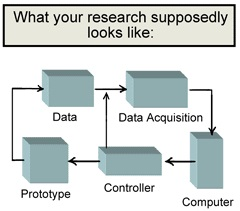
\includegraphics[width=.80\textwidth]{figuras/figura-1.jpg}
    \caption{\label{fig:exemplo-18}Exemplo.}
    
    Fonte: Exemplo%
\end{figure}
	
Integer non lacinia magna. Aenean tempor lorem tellus, non sodales nisl commodo ut. Proin mattis placerat risus sit amet laoreet. Praesent sapien arcu, maximus ac fringilla efficitur, vulputate faucibus sem. Donec aliquet velit eros, sit amet elementum dolor pharetra eget. Integer eget mattis libero.

Integer non lacinia magna. Aenean tempor lorem tellus, non sodales nisl commodo ut. Proin mattis placerat risus sit amet laoreet. Praesent sapien arcu, maximus ac fringilla efficitur, vulputate faucibus sem. Donec aliquet velit eros, sit amet elementum dolor pharetra eget. Integer eget mattis libero.


\section{Fundamentação Teórica B}
\label{sec:fundamentacao-teorica-b}

Integer non lacinia magna. Aenean tempor lorem tellus, non sodales nisl commodo ut. Proin mattis placerat risus sit amet laoreet. Praesent sapien arcu, maximus ac fringilla efficitur, vulputate faucibus sem. Donec aliquet velit eros, sit amet elementum dolor pharetra eget. Integer eget mattis libero. Praesent ex velit, pulvinar at massa vel, fermentum dictum mauris. Ut feugiat accumsan augue, et ultrices ipsum euismod vitae

\begin{figure}[htb]
    \centering
\includegraphics[width=.80\textwidth]{figuras/figura-2.jpg}
    \caption{\label{fig:exemplo-2}Exemplo.}
    
    Fonte: Exemplo%
\end{figure}

Nunc ac pretium dui. Mauris aliquam dapibus nulla ac mattis. Aenean non tortor volutpat, varius lectus vitae, accumsan nibh. Cras pretium vestibulum enim, id ullamcorper tortor ultrices non. Integer sodales viverra faucibus. Curabitur at dui lacinia, rhoncus lacus at, blandit metus. Integer scelerisque non enim quis ornare.

Duis faucibus, enim quis tincidunt pellentesque, nisl leo varius nulla, vitae tempus dui mauris ac ante. Quisque purus lorem, pharetra sit amet lobortis eu, vehicula vitae purus. Ut varius, erat nec vehicula elementum, risus est tempus justo, nec vulputate augue leo egestas metus.

\begin{figure}[htb]
    \centering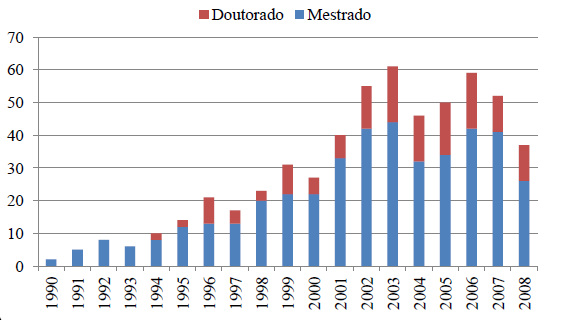
\includegraphics[width=.80\textwidth]{figuras/figura-3.png}
    \caption{\label{fig:exemplo-3}Exemplo.}
    
    Fonte: Exemplo%
\end{figure}

Integer non lacinia magna. Aenean tempor lorem tellus, non sodales nisl commodo ut. Proin mattis placerat risus sit amet laoreet. Praesent sapien arcu, maximus ac fringilla efficitur, vulputate faucibus sem. Donec aliquet velit eros, sit amet elementum dolor pharetra eget. Integer eget mattis libero.

\begin{table}[htb]
\centering
\caption{\label{tab:exemplo-tabela}Lista de trabalhos considerando as visualizações disponibilizadas}%
\resizebox{\textwidth}{!}{%
\begin{tabular}{|l|c|c|c|c|c|}
\hline
& \textbf{Sem Gráficos} & \textbf{Interatividade} & \textbf{Linha} & \textbf{Barra} & \textbf{Mapa de Calor} \\ \hline
Amershi e Conati                  &              & X              & X     &       & x     \\ \hline
Baruque et al.                    & X            &                &       &       &       \\ \hline
Bovo et al.                       & X            &                &       &       &       \\ \hline
Bravo e Ortigosa                  & X            &                &       &       &       \\ \hline
Chirioiu et al.                   &              & X              &       &       & X     \\ \hline
\end{tabular}
}
\end{table}
	
Duis faucibus, enim quis tincidunt pellentesque, nisl leo varius nulla, vitae tempus dui mauris ac ante. Quisque purus lorem, pharetra sit amet lobortis eu, vehicula vitae purus.